\documentclass[conference]{IEEEtran} % Usa la classe IEEEtran per formattazione simile

\usepackage{amsmath}
\usepackage{graphicx}



\begin{document}
\bstctlcite{IEEEexample:BSTcontrol}

\title{Exploring the Adversarial Robustness of AI-generated Image Detectors}

\author{
    \IEEEauthorblockN{Thomas Lazzerini, Samuele Cappelletti, Martina D'Angelo}
    \IEEEauthorblockA{
        University of Trento
    }
}

\maketitle

\begin{abstract}
Semi-supervised image classification is a machine-learning task in which a model is trained using a combination of labeled and unlabeled data. This paper consists of a high-level survey of semi-supervised image classification literature and expands on its main theoretical and practical challenges, providing a taxonomy of the most popular semi-supervised learning algorithms. ciao come va
\end{abstract}

\section{Introduction}
Semi-supervised image classification is nowadays a hot research topic. The objective is to tackle the major issue of Supervised Learning: the scarcity of labeled data...
% Continua con il tuo contenuto

As discussed in \cite{corvi2023detection}, semi-supervised learning is an important area of research.

\begin{figure}[h]
    \centering
    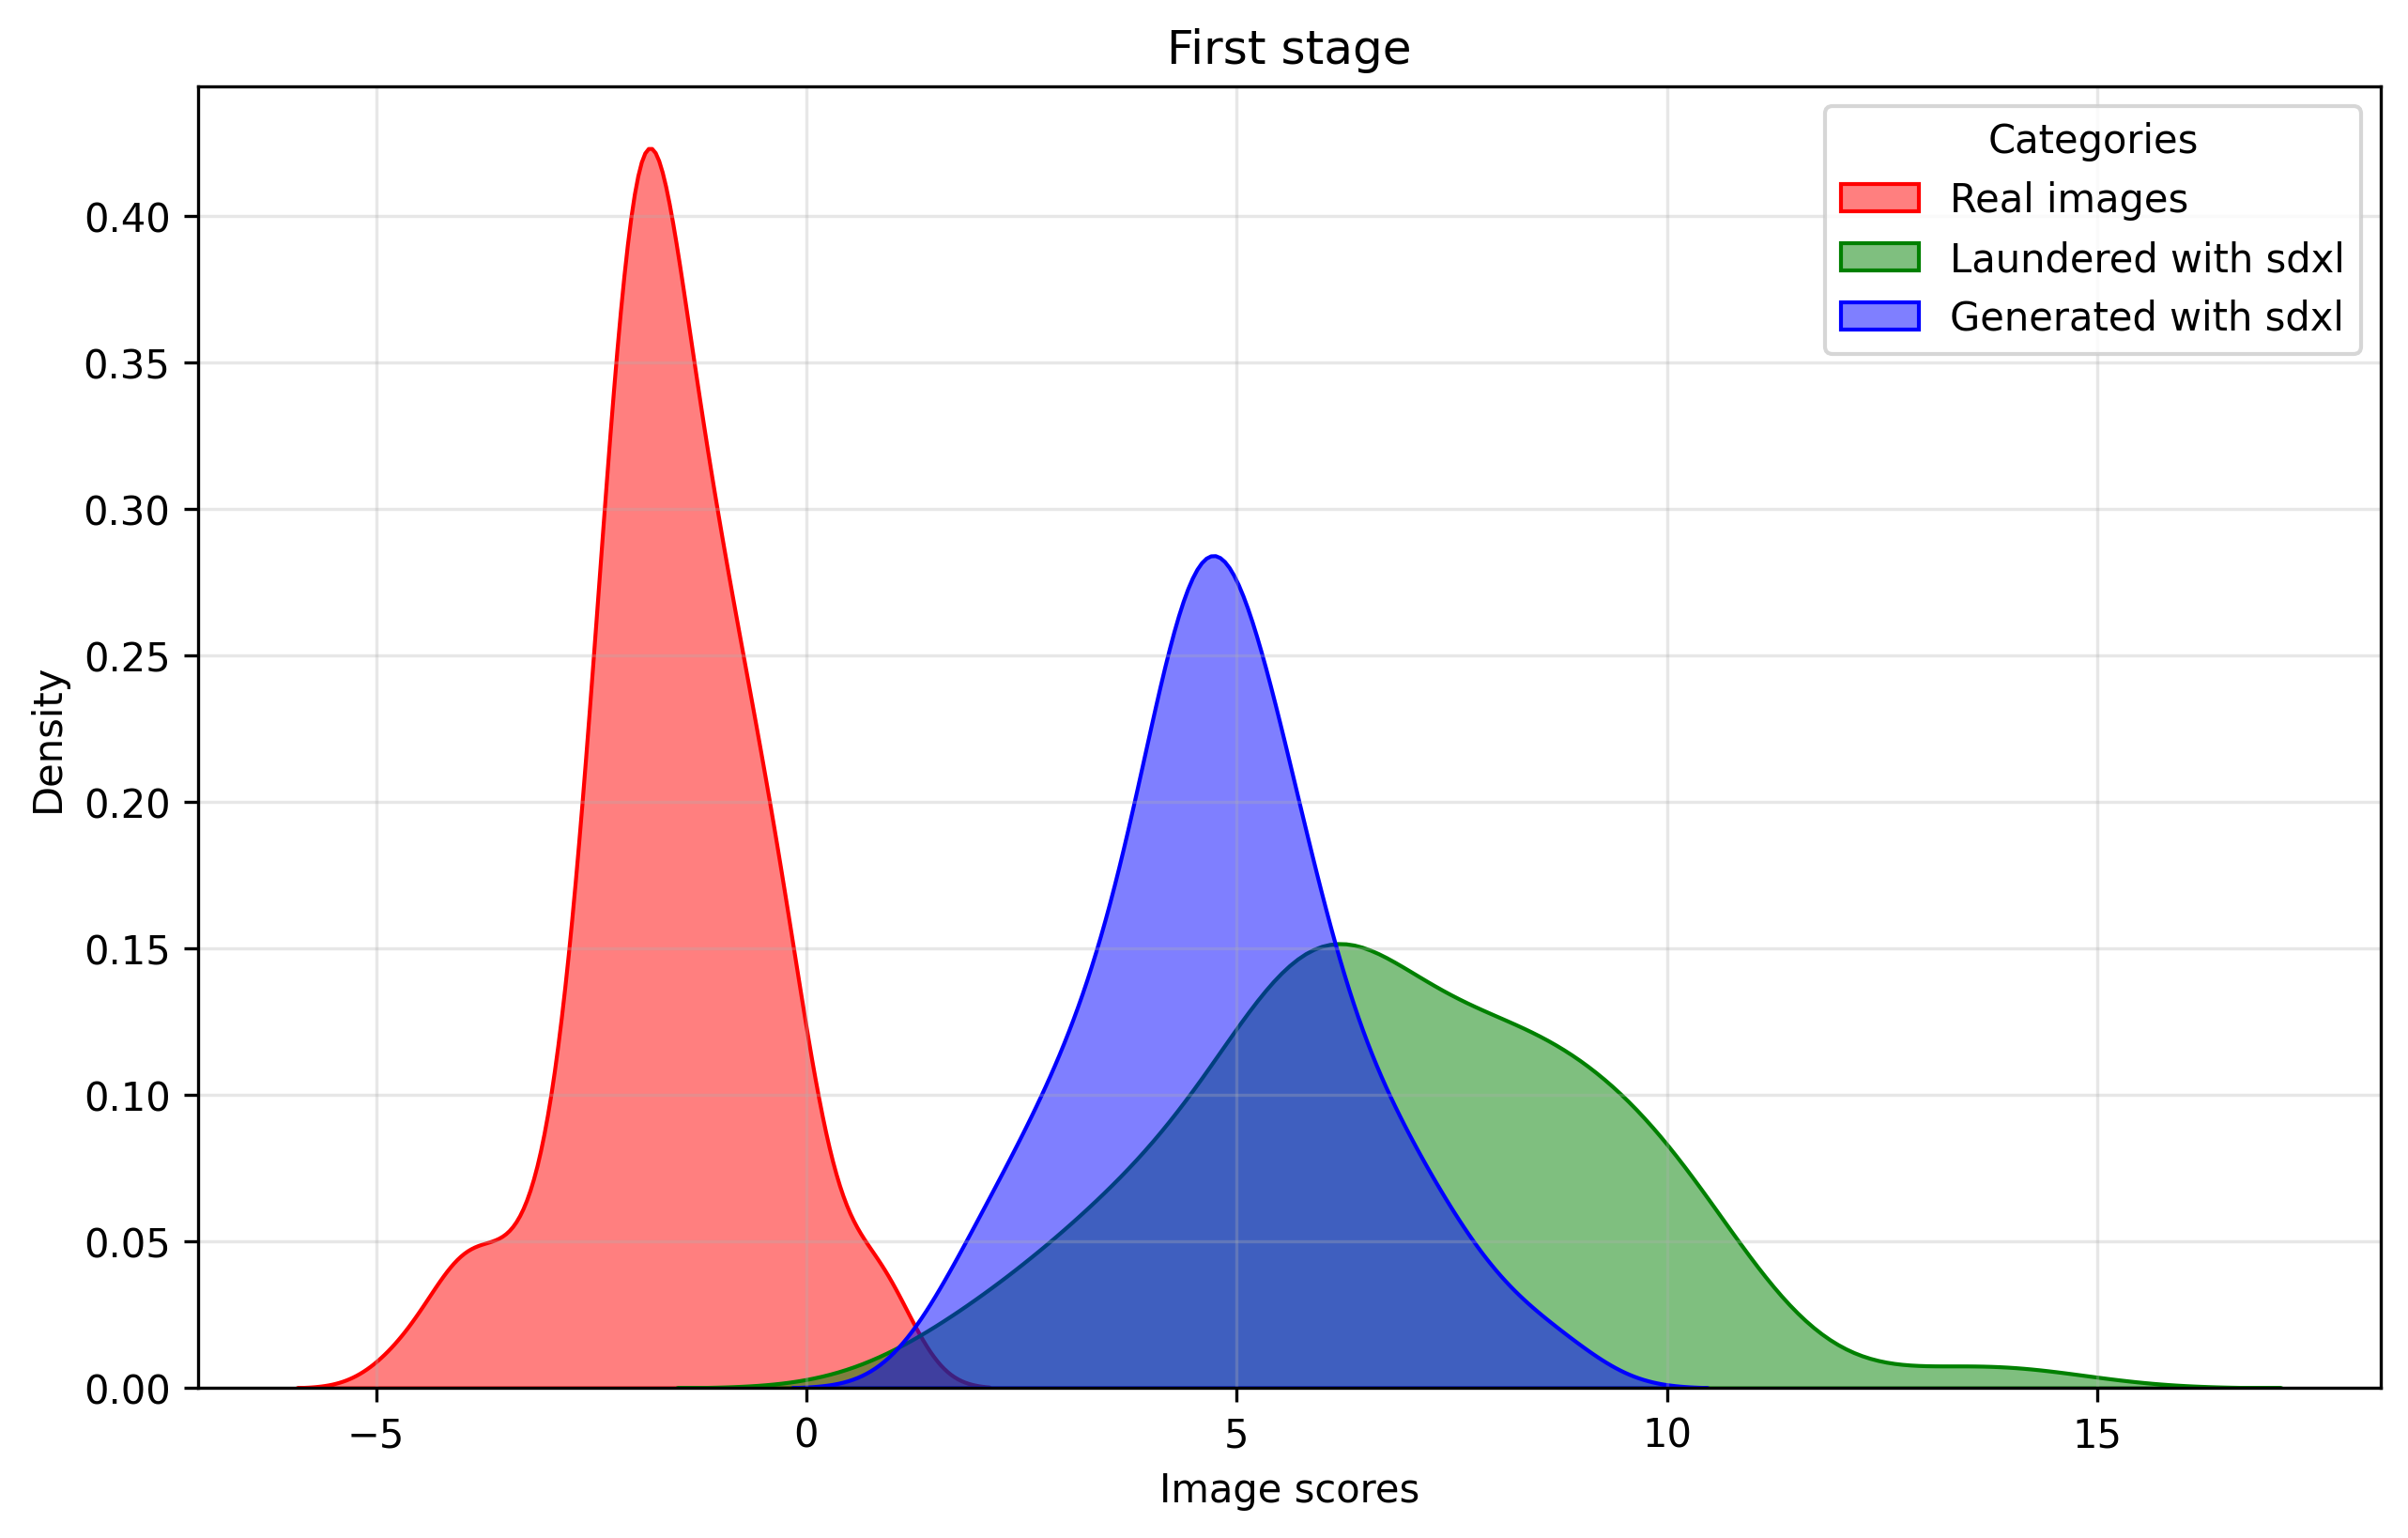
\includegraphics[width=0.8\linewidth]{Img/First_stage.png}
    \caption{Esempio di immagine.}
    \label{fig:esempio}
\end{figure}


\section{Detectors}
    \subsection{CLIP}
    \subsection{Detection of Images by Diffusion Models} 
        Lately, \textit{Diffusion Models} gained the spotlight in the image generation community, allowing for unmatched test-to-image photorealism and diversity. These new powerful tools are a new asset in the hands of malicious users, posing new challenges to the forensic community. Most SoTA detectors exploits low-level artifacts, not visible by a human eye, introduced during the generation phase by GAN generators. The study in \cite{corvi2023detection} suggests that, as can be seen in Fig. \ref{fig:pizza_fourier}, similar traces can be found also in DM-generated images

        \begin{figure}[h]
            \centering
            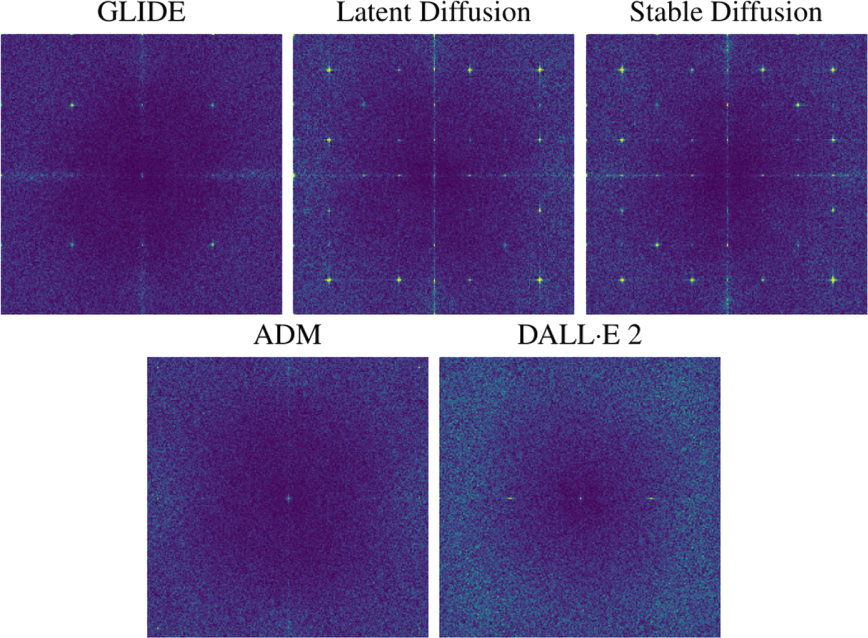
\includegraphics[width=0.6\linewidth]{Img/pizza_fourier.png}
            \caption{Fourier transform of of the fingerprint of some DM architectures (\textit{GLIDE} \cite{nichol2021glide}, \textit{Latent Diffusion} \cite{rombach2022high}, \textit{Stable Diffusion} \cite{stablediffusion2022}, \textit{ADM} \cite{dhariwal2021diffusion}, \textit{DALL$\cdot$E 2} \cite{ramesh2022hierarchical}) presented in \cite{corvi2023detection}}
            \label{fig:pizza_fourier}
        \end{figure}

        The study in \cite{corvi2023detection} also provides interesting evaluation results, comparing the performances of several SoTA detectors over different GAN and DM generators both in ideal case (uncompressed images) and real case (compressed and resized using the guidelines in \cite{vipcuplink}). These evaluations highlight how performances vary significantly between the models, due to the differences in their artifacts, therefore suggesting generalization difficulties (for example, in classifying a DM images with a GAN training and vice versa). Despite these difficulties, the inclusion of DM during training and performing an careful calibration procedure, like the one suggested by \cite{Platt1999probabilistic}, may help the generalization over similar architectures, despite not providing reliable results on out-of-training artifacts.
\section{Attacks}
    Despite the powerful detectors at our disposal, there exists many users that aim at attacking such detectors, in order to hide traces of their forgeries or also to introduce traces typical of generated images, to hide disguise content as fake. In the following chapter, some newly developed attacking techniques are discussed, to provide a general overview of the attacker-side.

    \subsection{Mimicry attack against image splicing forensic}
        As stated in \cite{boato2024adversarial}, this \textit{mimicry adversarial attack} can be used to hide image manipulation while forcing the detector to detect arbitrary ones by applying a gradient based optimization approach. Applied at large scale, this would cause high false-alarms, producing an effect similar to \textit{DoS} attacks while undermining the reliability of the target detector.

        The attack strategy proposed in \cite{boato2024adversarial} involves splitting the image in uniform patches and use these to compute a target representation for both the \textit{pristine patch $t_p$}, computed from the pristine patches, and the \textit{forged patch $t_f$}, computed from the forged patches. The function used for computing such target representations needs to be defined for each detector for the attack to be effective, this due to the fact that different detectors exploit different features. Once the targets have been computed, a gradient-based iterative approach is applied the each patch of the manipulated image, in order to make the patch feature representation more similar to the respective target's feature representation. A visualization of such iterative approach can be seen in Fig. \ref{fig:mim_visual}

        \begin{figure}[h]
            \centering
            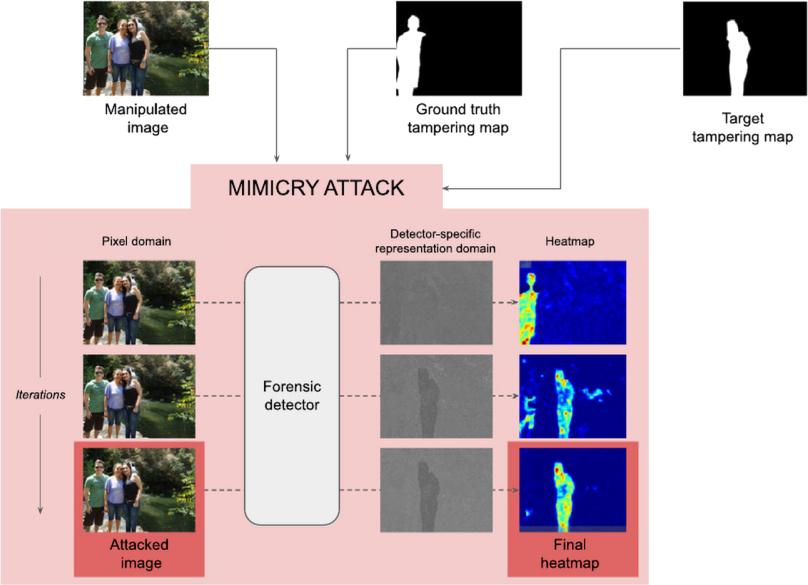
\includegraphics[width=0.8\linewidth]{Img/mim_visual.png}
            \caption{Visualization of the mimicry attack strategy and its effects proposed in \cite{boato2024adversarial}. The "\textit{ground truth}" tampering map represents the real forgery, while the "\textit{target}" tampering map represent the arbitrary forgery the attacker wants the detector to output}
            \label{fig:mim_visual}
        \end{figure}

        The evaluation results reported in \cite{boato2024adversarial} suggests this attack is highly effective, both in hiding the real forgery and also highlighting a "decoy" forgery arbitrarily introduced. Two image detectors were tested, \textit{Noiseprint} \cite{cozzolino2019noiseprint} and \textit{EXIF-SC} \cite{huh2018fighting}, over two different datasets, \textit{Columbia} \cite{ng2004data} and \textit{DSO-1} \cite{carvalho2015illuminant}. Several threshold-based and threshold-less metrics have been tested, with the latter being more important from the attacker point of view since the threshold values are unknown to him.

        Another interesting result presented in \cite{boato2024adversarial} regards the \textit{cross-detector} scenario, in which the attack is performed targeting a specific detector but then another is used in the evaluation. Also, \textit{stacked attacks} are considered, in which an image is sequentially attacked against different detectors. An evaluation in these regards reveal mixed results: a misaligned attack in not effective, while the performances of a stacked attack are highly dependant on both the order of the attacks and the detector used in the evaluation. Nevertheless, this is an interesting scenario open for further studies.

    \subsection{Image Laundering with Stable Diffusion}
        \label{sec:laundering}
        Differently from "classic" diffusion models, like \textit{Latent Diffusion}, \textit{Stable Diffusion} models allow the users to provide an initial image as input \cite{sd1_github} \cite{sd2_github} \cite{podell2023sdxl} \cite{sauer2023adversarial-sdxl-turbo}. This image will be superimposed with noise and modified by the model according to the textual prompt. The weight of such modifications can be set via a dedicated strength parameter in the range $[0, 1]$.

        Processing images in such pipeline using a strength parameter equal to 0 produces outputs with the maximum similarity to the inputs: the image is encoded and decoded right away, without any denoising step. As suggested in \cite{mandelli2024synthetic}, this process could be exploited by malicious users in order to mask real content as synthetic. In fact, the encoding/decoding is sufficient to introduce enough artifacts into the real image to make it synthetic in the eyes of numerous detectors. This practice is known as \textit{image laundering}.

        The study in \cite{mandelli2024synthetic}, proposes a two-step architecture, visualized in Fig. \ref{fig:launder_2_stage}, as solution to efficiently discriminate between real, fully synthetic and laundered images. Such architecture is inspired by \cite{mandelli2022detecting}, in which the image is split into multiple random patches, a score is assigned to each one and the average o the highest scores provide the global score of the image: a positive score suggest a synthetic image, while a negative score a real one. Despite the good results, this backbone architecture alone is unfit for the laundered image detection task, hence the introduction of the 2 steps: the first step discriminate real from synthetic images, while the second step discriminate fully synthetic from laundered images.

        \begin{figure}[h]
            \centering
            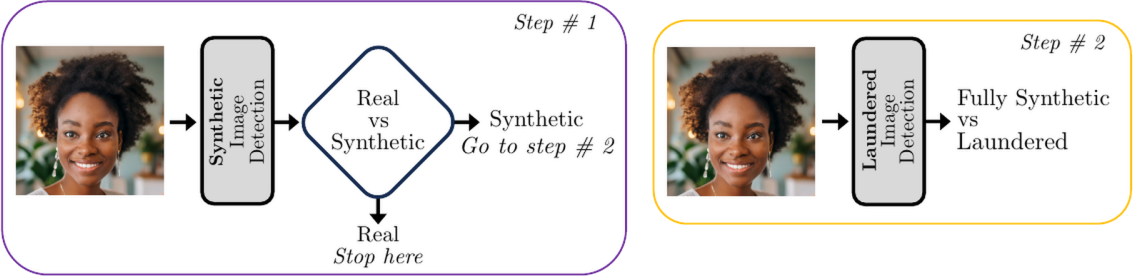
\includegraphics[width=0.95\linewidth]{Img/launder_2_stage.png}
            \caption{Visualization of the 2 step architecture proposed in \cite{mandelli2024synthetic} for the laundered image classification task. The first step discriminate real images from synthetic (both fully and laundered) ones, while the second step discriminate fully synthetic images from laundered ones}
            \label{fig:launder_2_stage}
        \end{figure}

        The evaluation provided in \cite{mandelli2022detecting} about such 2 step pipeline are good: the first step reach a good separability between real and synthetic image, while the second step reach almost perfect results over multiple models and multiple metrics, with only minor decreases in performances when post-processing operations like JPEG compression and resize are applied.
    \subsection{Adversarial Robustness}
\section{Experiment}
    In this first phase of the project, our team executed a preliminary experiment, to asses the capability of the laundering attack, from the section \ref{sec:laundering}, on the dataset \textit{TrueFake} provided by the \textit{MMLAB} team.

    The first phase of the experiment consisted in recovering 25 real images and, given their large size, extract 4 patches of size $1024\times1024$ from each of them, for a total of 100 real patches. Next, such patches were laundered, with a \textit{denoising} parameter of 0, using the model \textit{sd\_xl\_base\_1.0} \cite{sdxl_base_1_0}. Lastly, a total of 100 fully synthetic images, generated by \textit{Stable Diffusion XL}, were collected from the \textit{TrueFake} dataset in equal quantity from each category available.

    This small dataset was submitted to the 2 step pipeline from \cite{mandelli2024synthetic}, visualized in Fig. \ref{fig:first_stage}, obtaining interesting results. The first step, as can be seen in Fig. \ref{fig:first_stage},  yielded similar results as \cite{mandelli2024synthetic}, with a good separability around threshold 0. On the other hand, the second step, in Fig. \ref{fig:second_stage}, yielded results slightly different from \cite{mandelli2024synthetic}, in particular the fully synthetic images had a average score of about 1, where \cite{mandelli2024synthetic} reported good separability at threshold 0. 

    \begin{figure}[h]
        \centering
        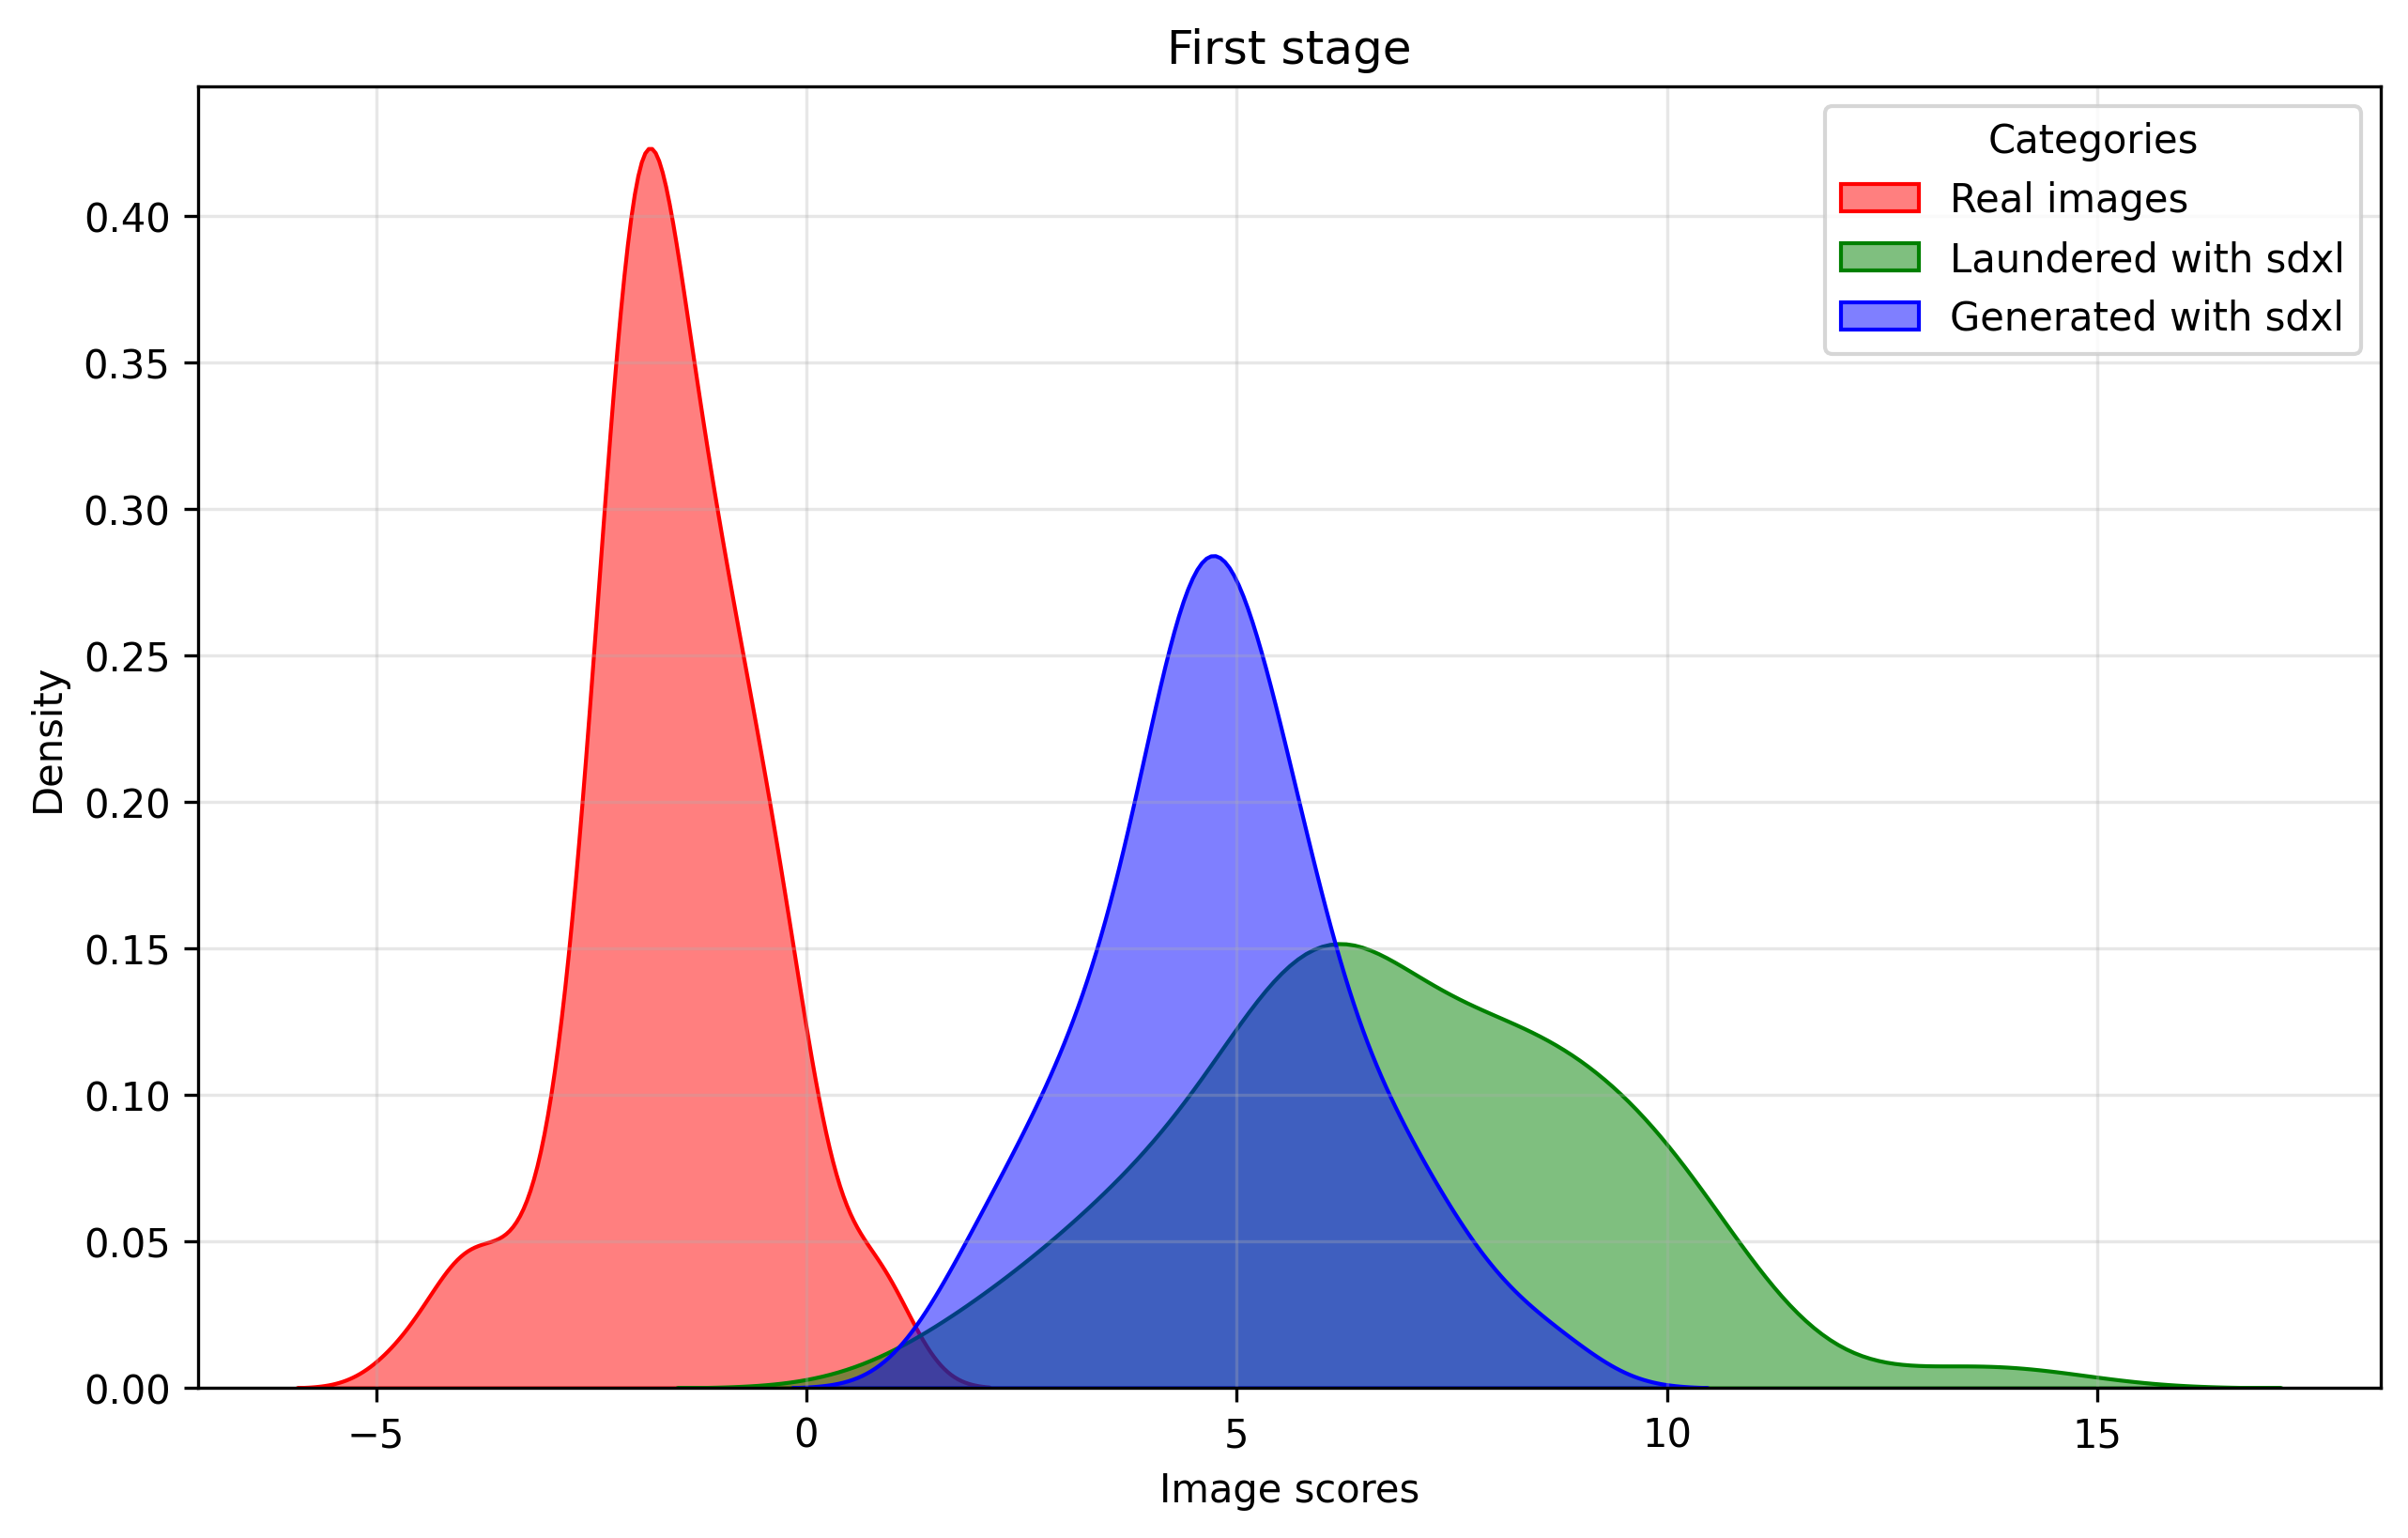
\includegraphics[width=0.95\linewidth]{Img/first_stage.png}
        \caption{Results of the first step of the pipeline from \cite{mandelli2024synthetic} using images from \textit{MMLAB TrueFake} dataset}
        \label{fig:first_stage}
    \end{figure}

    \begin{figure}[h]
        \centering
        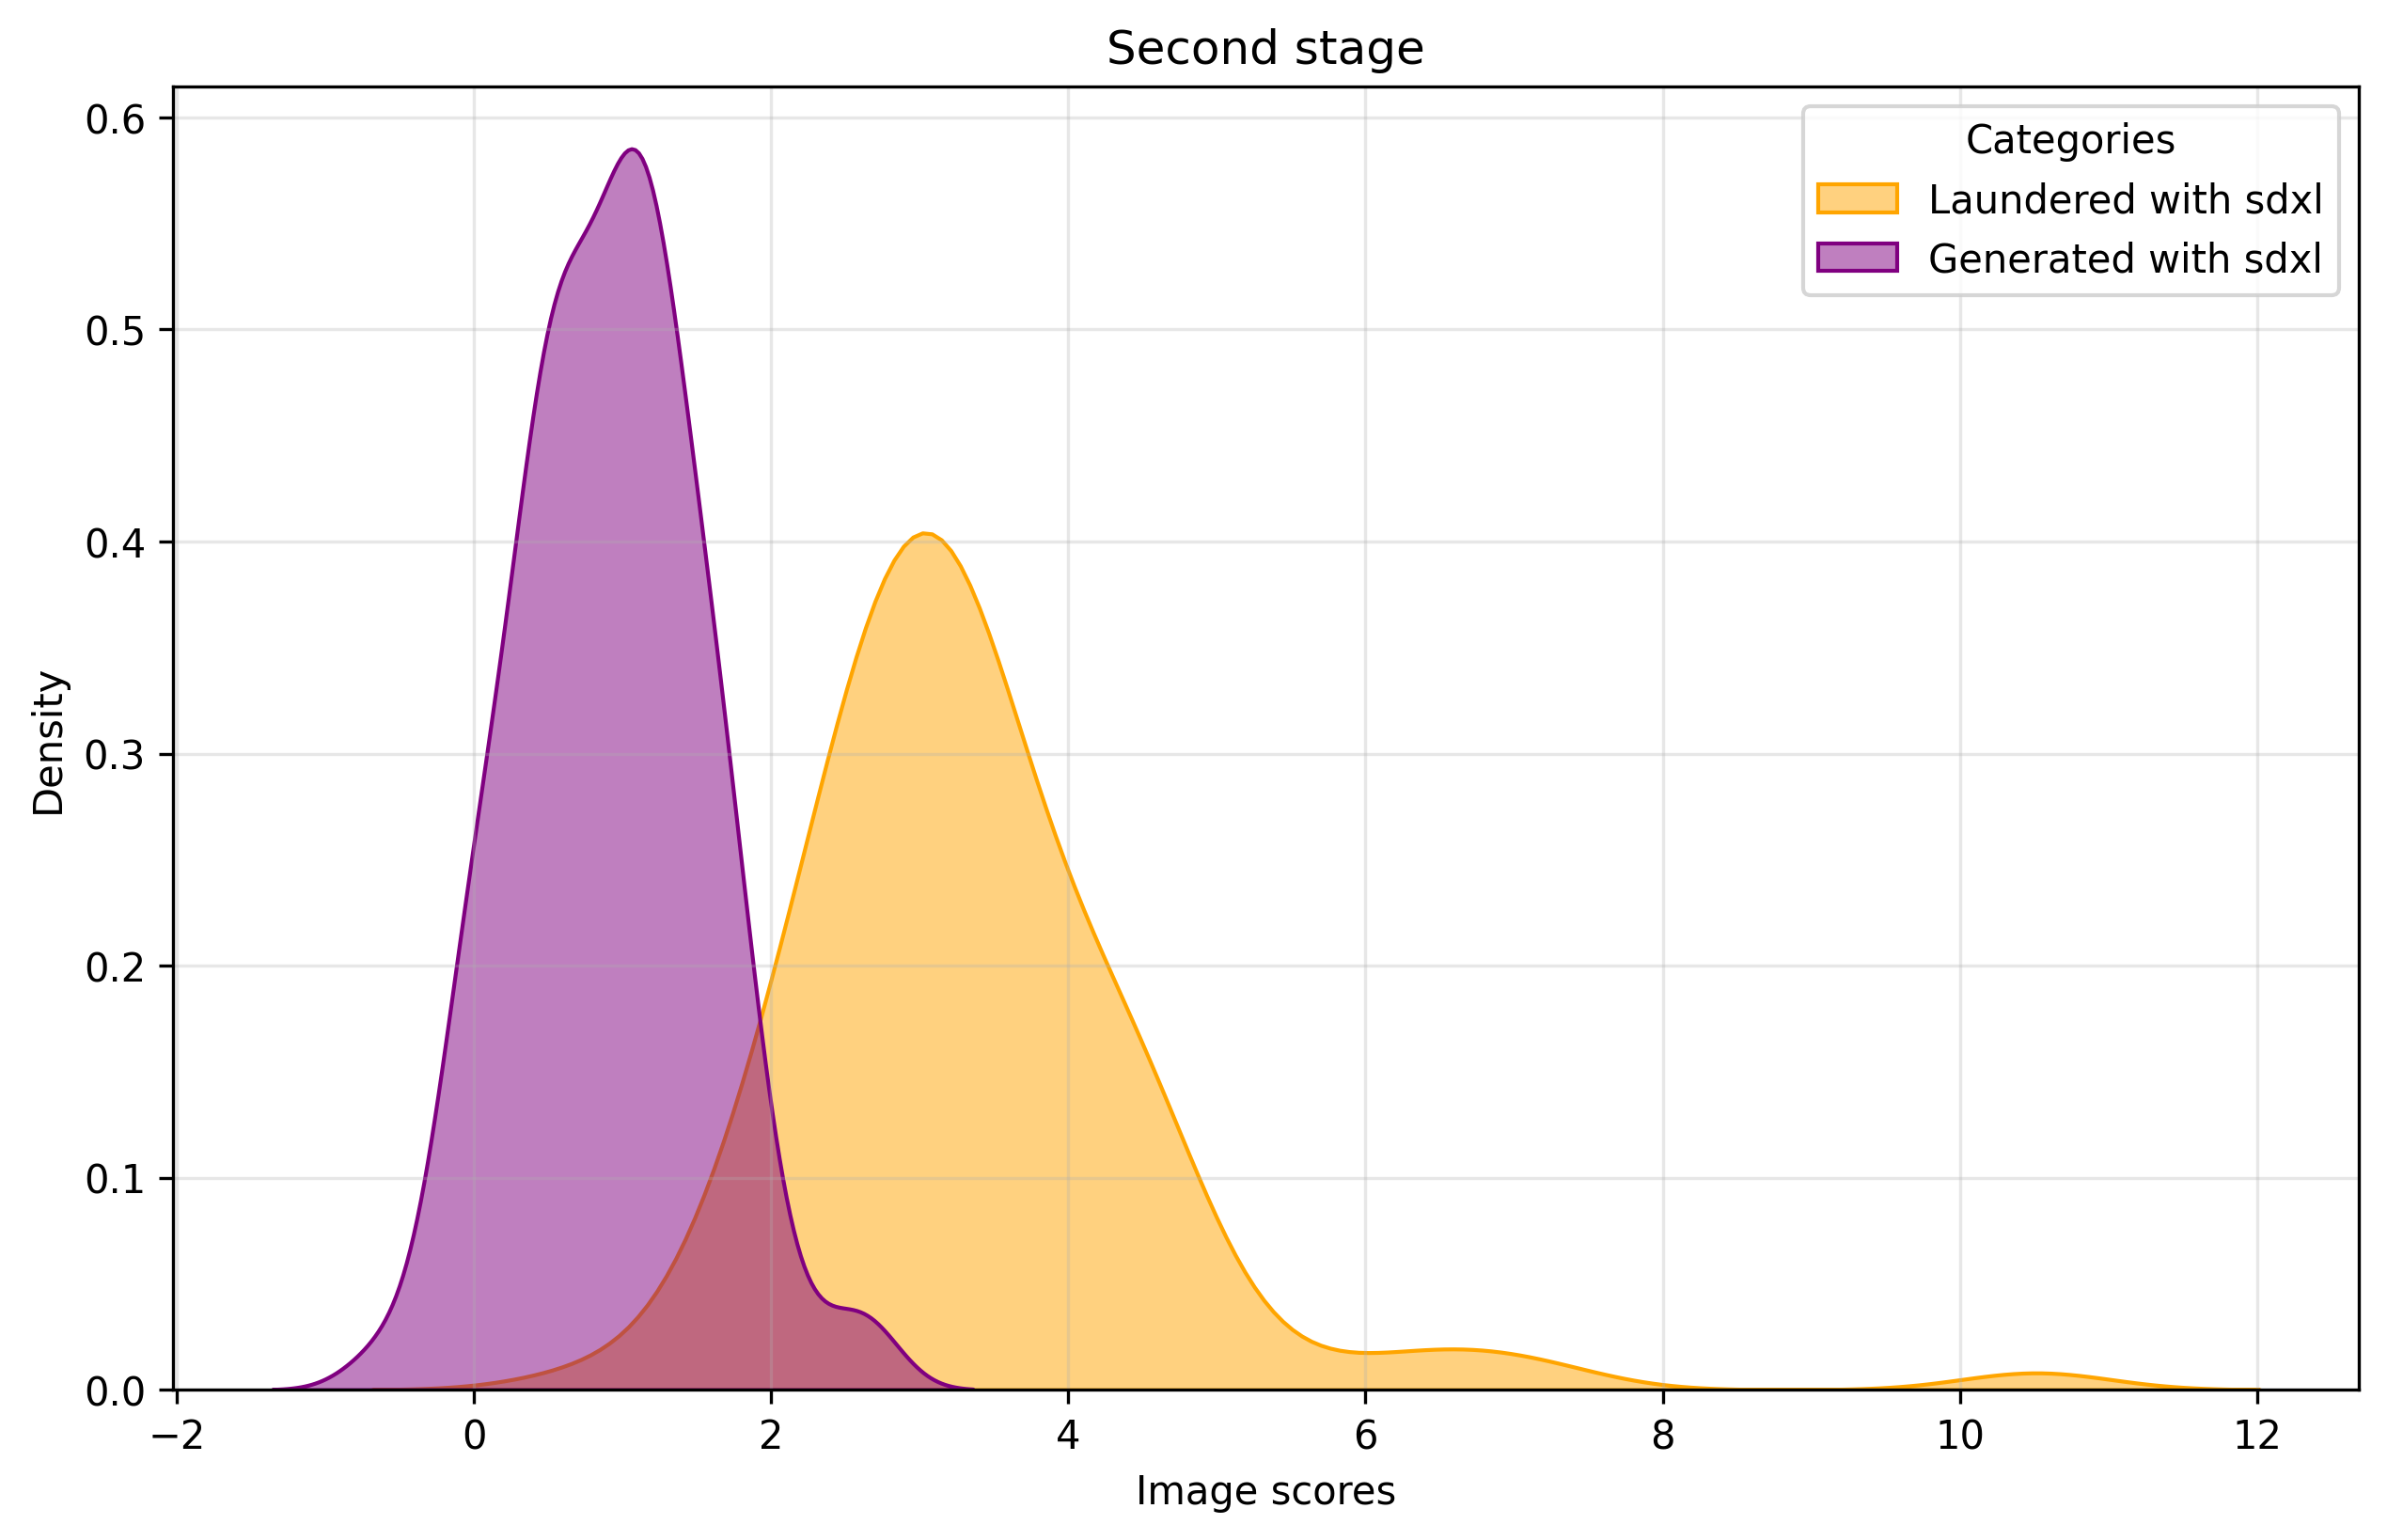
\includegraphics[width=0.95\linewidth]{Img/second_stage.png}
        \caption{Results of the second step of the pipeline from \cite{mandelli2024synthetic} using images from \textit{MMLAB TrueFake} dataset}
        \label{fig:second_stage}
    \end{figure}
\section{Conclusions}

\bibliographystyle{IEEEtran} % Stile delle referenze (es. IEEE)
\bibliography{references}    % Nome del file .bib (senza estensione)

\end{document}